\pagelayout{margin}
\setchapterstyle{kao}
\setchapterpreamble[u]{\margintoc}
\chapter{Related research}

\todo[inline]{The introduction to this chapter needs significant improvement. The current text is informal and contains grammatical errors. Rewrite to provide a clear, structured overview of the literature review approach and organization. Use complete sentences and academic language.}

This section mentions relevant literature that focuses either on the very same issue. Or topics close to predicting EV charger demand. There are not that many papers focusing on our specific issue however there is a lot of knowledge ihdden inside of them. The papers analyzed in this chapter provide insight into how similar issues were tackled. And on what does the research focus on.


First, from an outside perspective. Issues and topic of the papers will be explored. What outcome were they focused on. And then an inside look, into what research approaches they took and what methods were used.

Because this is spatial data science. Most of the papers are very practical in a sense that they work with real datasets. And each country and even city has different data gathering culture and data availabilty. The research is tightly connected to what data is available. No relevant paper for our issue was found focusing on Prague.

\todo[inline]{This chapter should begin with a clear explanation of your literature review methodology - how papers were selected, what databases were searched, what inclusion/exclusion criteria were used, and how many papers were ultimately reviewed.}


\section{Issue addressed}

\todo[inline]{This section title should be more descriptive, such as "Key Research Areas in EV Charging Literature". The current bullet list should be expanded into proper paragraphs that explain each research area and how they relate to your work.}

\begin{itemize}
    \item EV charger demand prediction
    \item EV charger use anaylsis \todo[inline]{Spelling error: "anaylsis" should be "analysis"}
    \item Charging infrastructure planning and optimization
    \item Digital twin
\end{itemize}

\section{Research approaches}

\todo[inline]{This section is extremely underdeveloped and informal. It should be completely rewritten to provide a comprehensive overview of the different methodological approaches in the literature, with proper citations and explanations of how each approach contributes to the field.}

Starting from simple statistics. Then menitoning agent simulations. And end with ML.

Research applies itself to all sorts of EV stuff. Starting from understanding coverage of existing EV chargers.

\subsection{Understanding EV Charger Use by Data}

To understand why certain chargers are being utilized the way they are. Research utilizes traditional and Bayesian statistics. As the person that plans \acrfull{CP} it is good to have insight into what influences charging demand. That is, why a certain charger is utilized. And what factors contribute to it. So far, we dont care about expansion of the infrastrcture. But could provide insights that allow to place new chargers more strategically.

\sidecite{hechtGlobalElectricVehicle2024} gathered counts of types of \acrfull{POI}\sidenote{types like shops, sport areas, schools, offices} near every charger of interest \sidenote{Search radius of 2000m around each charger with linear decrease in importance in relation to distance} from Open Street maps. Then for each charger computed its utilization. Which is its average daily power consumption. Then used linear regression to test which of the category of \acrfull{POI} contributed to the consumption.
The study had some statisficaly significant results. They also trained neural network model for capturing non linear relationships. User can use the model to select any point where a \acrfull{CP} might be placed and see its estimated utilization and evaluate worthiness of placement. However it does not work with other chargers in the area and does take into account charger density. The paper has identified that certain categories of \acrfull{POI}\sidenote{\acrshort{POI} data obtained from OpenStreetMaps} are correlated with charger demand.

\sidecite{dongElectricVehicleCharging2019} uses log-Gaussian Cox process. Which is a statistical model that can handle dependence between points on a map (EV chargers). It has identified that workplace population and traffic flow are positively related to demand of\acrfull{CP} while commerce is in a negative relation. \sidenote{<workplace population, traffic flow, commerce description here>}.

\begin{kaobox}[frametitle=Simulation vs Model]
    Model is concerned with representing a system of interest. Purpose of it is so it matches its real system in some behaviour while being simpler than reality. There are many ways how to construct models. From simplest small replicas (small car models to use in wind tunnel) to complicated mathematical and software ones.

    Simulation is then a use of model to try to replicate some real system of interest to gain insights how a real system might behave .

    An example can be a toy car and a ramp which would be our model. Then pushing the car off the ramp to see how far it is able to land. This is much less expensive than pushing real cars of larger ramps.

    \cite{maria1997introduction}
\end{kaobox}

\subsection{Simulations and EV Charger Use}

\textbf{Trafic models} are used to estimate \acrfull{CP} demand. They are a mathematical model of real-world trafic. And they can estimate charging demand by introducting EV vehicle agents into the simultion. Those agents navigate replica of real road network. While also being able to emulate traffic jams, alternative path finding. Negative of these models is that they are harder to develop, fine tune to match real situation. And performance costly. But once developed and validated with real-world. They can be highly utilized.

\begin{kaobox}[frametitle=\text{Micro,Macro,Meno-Scopic}]

    Traffic models can be separated into three groups according to \cite{TrafficAnalysisTools}\cite{HomeAustroads}(\cite{lachowiczMicroscopicMesoscopicMacroscopic2011} also writes about splitting simmulation models into 3 groups with a more theoretical view):

    % \todo{improve, im actually not really sure about the difference of mesoscopic vs rest}
    \begin{itemize}
        \item \textbf{Microscopic} - Simulation of individual agents/vehicles. Can be as detailed as emulating accelerating, lane changing, turning. Higher fidelity isuUsable for example when designing intersection with light signals optimizing for traffic or pedestrian flow. But the model can also have less detailed fidelity for vehicles. Which simplifies the simmulation and enables larger area of interest. Like cities or even countries.
        \item \textbf{Mesoscopic} - Provide less fidelity than microscopic. improve
        \item \textbf{Macroscopic} - Work with aggregate information. Work more on analytical model and proven mathematcial relationships between traffic flow. improve
    \end{itemize}
\end{kaobox}


Matsim \sidecite{communityMATSim2025} is \acrfull{ABM} \marginnote{Slight foreshadowing but this approach was not taken in this thesis however it was considered.}. It's OpenSource software licensed under GPLv2, implemented in Java. And started in 2004 in Zurich. It falls into category of microscopic models due to it being able to simluate individual agents. The model simmulates simplifed version of vehicle movement and traffic which is needed to correctyl simulate entire city including congestions. The simulation usually concerns only one day. To create such a model the following are needed:
\begin{itemize}
    \item \textbf{Road/communication Network} - Spatial data for area of interest reagarding: roads, intersections, tram or train tracks etc. Obtained from technical data published by goverments or third party map providers. (Mainly OpenStreetMaps)
    \item \textbf{Population} - Agents with their day plan, where are they going to live and commute to work. Those are generated with help of expert knowledge and travel diaries survey.
    \item \textbf{Facilities} - Locations where activities can be performed. Obtained from third parties like OpenStreetMaps.
\end{itemize}

\begin{figure}
    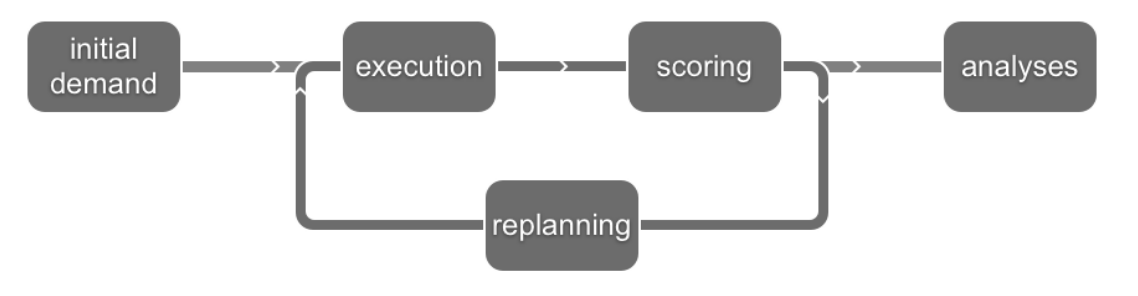
\includegraphics{matsim-simmulation-stages.png}
    \caption[Matsim, Simulation stages]{Stages of matsim simulation. \cite{Horni2016}}
    \labfig{matsim-simulation}
\end{figure}

The agents plan assigns unique daily schedule for each agent in the population. See \ref{fig:matsim-simulation} This estabilished the initial demand. During the execution step, Matsim simulates agents commute and tries to satisft the agents schedule. The agent might fail to be on schedule due to road or public transport congestion from other agents. After finishing the simulation the agents actual daily schedule is scored. Penalizing arriving at work late or being stuck for too long in traffic giving agents lover score. While agents who got where they wanted qucikly and without trafic jams get better score. During replanning agent schedule can be modified so it either adjusts the agents schedule, like less time spent home or taking a different route to work. When the simulation is sufficiently optimized the results of it can be then used for various analysis as the output of the modle is detailed log of agent activities.

\begin{marginfigure}
    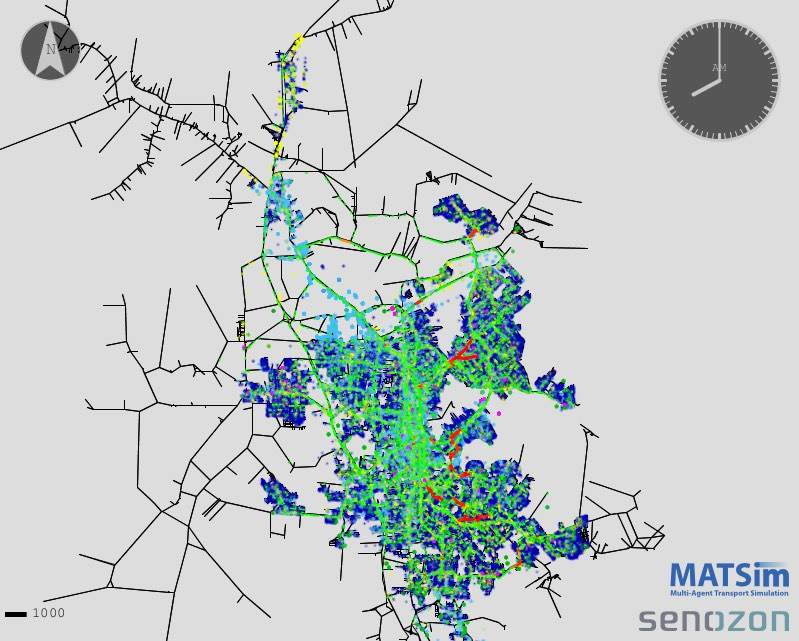
\includegraphics{joinville_1.jpg}
    \caption[Matsim, Joinville example]{Matsim, Joinville example. Model intended to help the city encumbered by high traffic volumes.\\
        \url{https://matsim.org/gallery/joinville/}}
    \labfig{joinville_example}
\end{marginfigure}

To create the agents schedule, day intentions need to be provided to the model. Those can be either manually crafted. With the increased availabiliy of census data, data driven approach can be taken. This trades away the possibility to experiment with different kinds of populations and policies\sidenote{like exmaining effect of different school time start on traffic} but simplifies the process of creation where only data is needed and not expert knowledge on human behavior. \sidecite{drchalDatadrivenActivityScheduler2019} models multiple probability densities for what activity will an agent do, how long it will take and what activities are available in the area. This utilizies several datasets. New schedules can be generated from the model by sampling from the distributions.

Finaly, moving to use of Matsim for ev scenarios. \sidecite{novoselAgentBasedModelling2015} studies the impact of EVs on the electric id and electricty production in Croatia. By having a simmulation of power production network for the whole country as well. They first have a simmulation regarding the current state and how that impacts the electrical grid. This sets the baseline and also allows to correctly calibrate the model. Then they increase the ev adoption and see what is the hourly energy consumption of EVs and their impact on the grid.

\todo{Talk about arup}

\textbf{Stochastic models} provide a way for modeling charging behavior of electric vehicles by capturing randomness and uncertainty in travel patterns. They work with more simplified representation fo reality compared traffic models\sidenote{Of course trafic models have large part of stochasticity inside themselves}. These models typically employ probability distributions to characterize variables such as departure times, travel distances, parking durations, and charging decisions. By sampling from these distributions using techniques like Monte Carlo simulation, they generate synthetic power demand profiles.

\sidecite{bradyModellingChargingProfiles2016} presents an example of stochastic modeling applied to EV charging behavior. Their approach uses a non-parametric copula function to model the dependence structure between six variables: departure time, number of journeys, and total distance traveled across two consecutive days. For this they utilize real-world GPS data collected from electric vehicles. Their model simulates complete journey schedules for individual vehicles and implements a probabilistic charging decision model at each destination, conditioned on the state of charge, parking time, and journey number. The approach captures the variability in charging behavior by incorporating factors such as battery characteristics and probabilistic charging point availability.

Paper: \sidecite{ul-haqProbabilisticModelingElectric2018}
\todo{probably skip, the paper is too hard}
\begin{itemize}
    \item tests policy changes
    \item estimate ev charging pattern based on residents activity patterns
    \item utilizes markov chain to estimate next trip departure time and travel distance
    \item does not have charging data, so from simmulation of a day it guesses how much the ev needs to be charged
    \item graphical model with good diagram/description
\end{itemize}



Paper: \sidecite{powellScalableProbabilisticEstimates2022}
\begin{itemize}
    \item groups drivers hiearrchicaly by charging behaviour
    \item utilization of actual charging data, charging sessions data. In the session, driver id is available. So drivers charging behaviour can be observed.
    \item utilize monte carlo simulation. Sample from learnt prob distributions.
    \item validated against real data
    \item $P(s,z,G) = P(s|z,G)\;P(z|G)\;P(G)$
\end{itemize}


\begin{itemize}
    \item \sidecite{ul-haqProbabilisticModelingElectric2018}
    \item \sidecite{zhangChargingDemandPrediction2023}
    \item \sidecite{zhangUrbanChargingLoad2024}
\end{itemize}


\section{Forecasting}
\todo{mention difference forecasting vs modelling}

\textit{ML for predictions, not explainable. Just learning on data}

\todo[inline]{This section contains only placeholder text and a todo note. It needs to be fully developed with a comprehensive review of forecasting approaches in EV charging demand literature, including both statistical forecasting methods and machine learning approaches. Include a discussion of the trade-offs between model explainability and predictive performance.}

\section{Infrastructure Planning}

\textit{Charger placement, optimization problem how to cover certain areas. ILP and others used}

\todo[inline]{This section also contains only placeholder text. Develop a comprehensive review of infrastructure planning approaches, including optimization methods, coverage models, and decision support systems. Discuss how these approaches relate to your research on charging demand prediction.}


\section{Czechia and Prague Relevant Research}

\textit{No research paper has been found with theme of EVs and Czechia/Prague. So only relevant stuff is gonna be mentioned}

\todo[inline]{This section needs to be developed beyond placeholder text. Even if no direct research on EV charging in Prague exists, you should discuss relevant research on urban mobility in Prague, transportation planning in Czech cities, or other related topics that provide context for your work. The citations listed need to be properly discussed, not just listed.}

\sidecite{pekarekModelChargingService2017}
\sidecite{elomiyaAdvancedSpatialDecision2024}
\sidecite{uglickichPoissonbasedFrameworkPredicting2025}

\section{Data sources and transformations}
estimate population

Predicts density of each building per $100m^2$ living area. With $R^2 = 94\%$.
\sidecite{shangEstimatingBuildingscalePopulation2021}

\section{Discussion}

\todo[inline]{This discussion section needs significant improvement. It should synthesize the findings from the literature review, identify research gaps, and clearly position your work within the existing literature. The current text is informal and lacks proper structure.}

From observed papers regarding simulation to obtain some estimate of charging demand. Either, in absence of data, expert knowledge is utilized to create simmulations. Which lean more on engineering complexity. Due to need to simmulate some percent of city/country population. But they might not always be feasible to develop as well as calibrating. Which is to ensure the simulation matches real world. But then they have large utility and flexibilty. For example examine policy changes.

When data is available, turn to more data based methods is more common. Instead of microscopic simulations. Stochastic properties of people are obtained from the data or estimated to match the data.

\section{Research gaps}

\textit{Mention how the relevant research is helpful for us. Also how noone has studied Prague and that it has different data landscape. And so we have to do a new approach.}

\todo[inline]{This section contains only placeholder text. It should be fully developed to clearly articulate the specific research gaps your work addresses. Explain how your approach differs from existing methods and why it's necessary given the unique context of Prague. This section is crucial for establishing the novelty and contribution of your research.}

\todo[inline]{Overall, this entire chapter needs substantial development. Many sections contain only placeholder text or brief notes. A thorough literature review is essential for positioning your research within the existing body of knowledge and establishing its contribution. Each section should be expanded with proper academic writing, comprehensive analysis of relevant papers, and clear connections to your research objectives.}
